\documentclass{standalone}
\usepackage{tikz}
%\usetikzlibrary{...}
\usepackage{siunitx}
\begin{document}
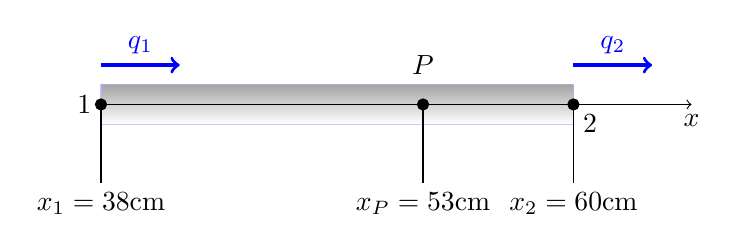
\begin{tikzpicture}[scale=1]
	\shadedraw[color=blue!30, opacity=.7] (0,-.25) rectangle (6, .25);
	\draw[->, thin] (0, 0) -- (7.5, 0) node[below]{$x$};
	\draw[fill=black] (0,0) circle (2pt) node[left]{$1$};
	\draw[fill=black] (6,0) circle (2pt) node[below right]{$2$};
	
	\draw[fill=black] (4.09,0) circle (2pt);
	\node at (4.09, .5) {$P$};
	
	\draw[thin] (0,0) -- (0,-1) node[below]{$x_1=38\unit{cm}$};
	\draw[thin] (4.09,0) -- (4.09,-1) node[below]{$x_P=53\unit{cm}$};
	\draw[thin] (6,0) -- (6,-1) node[below]{$x_2=60\unit{cm}$};
	
	\draw[->, very thick, blue] (0, .5) -- (1, .5) node[pos=.5, above]{$q_1$};
	\draw[->, very thick, blue] (6, .5) -- (7, .5) node[pos=.5, above]{$q_2$};
\end{tikzpicture}
\end{document}